\documentclass[hyperref, a4paper]{article}

\usepackage{geometry}
\usepackage{float}
\usepackage{titling}
\usepackage{titlesec}
% No longer needed, since we will use enumitem package
% \usepackage{paralist}
\usepackage{enumitem}
\usepackage{footnote}
\usepackage{enumerate}
\usepackage{amsmath, amssymb, amsthm}
\usepackage{mathtools}
\usepackage{bbm}
\usepackage{cite}
\usepackage{graphicx}
\usepackage{subcaption}
\usepackage{physics}
\usepackage{tensor}
\usepackage{siunitx}
\usepackage{booktabs}
\usepackage[version=4]{mhchem}
\usepackage{tikz}
\usepackage{xcolor}
\usepackage{listings}
\usepackage{autobreak}
\usepackage[ruled, vlined, linesnumbered]{algorithm2e}
\usepackage{xr-hyper}
\usepackage[colorlinks,unicode]{hyperref} % , linkcolor=black, anchorcolor=black, citecolor=black, urlcolor=black, filecolor=black
\usepackage{prettyref}

% Page style
\geometry{left=3.18cm,right=3.18cm,top=2.54cm,bottom=2.54cm}
\titlespacing{\paragraph}{0pt}{1pt}{10pt}[20pt]
\setlength{\droptitle}{-5em}
\preauthor{\vspace{-10pt}\begin{center}}
\postauthor{\par\end{center}}

% More compact lists 
\setlist[itemize]{itemindent=17pt, leftmargin=1pt}

% Math operators
\DeclareMathOperator{\timeorder}{\mathcal{T}}
\DeclareMathOperator{\diag}{diag}
\DeclareMathOperator{\legpoly}{P}
\DeclareMathOperator{\primevalue}{P}
\DeclareMathOperator{\sgn}{sgn}
\newcommand*{\ii}{\mathrm{i}}
\newcommand*{\ee}{\mathrm{e}}
\newcommand*{\const}{\mathrm{const}}
\newcommand*{\suchthat}{\quad \text{s.t.} \quad}
\newcommand*{\argmin}{\arg\min}
\newcommand*{\argmax}{\arg\max}
\newcommand*{\normalorder}[1]{: #1 :}
\newcommand*{\pair}[1]{\langle #1 \rangle}
\newcommand*{\fd}[1]{\mathcal{D} #1}
\DeclareMathOperator{\bigO}{\mathcal{O}}
\DeclareMathOperator{\object}{Ob}
\DeclareMathOperator{\morphism}{Hom}

% TikZ setting
\usetikzlibrary{arrows,shapes,positioning}
\usetikzlibrary{arrows.meta}
\usetikzlibrary{decorations.markings}
\tikzstyle arrowstyle=[scale=1]
\tikzstyle directed=[postaction={decorate,decoration={markings,
    mark=at position .5 with {\arrow[arrowstyle]{stealth}}}}]
\tikzstyle ray=[directed, thick]
\tikzstyle dot=[anchor=base,fill,circle,inner sep=1pt]

% Algorithm setting
% Julia-style code
\SetKwIF{If}{ElseIf}{Else}{if}{}{elseif}{else}{end}
\SetKwFor{For}{for}{}{end}
\SetKwFor{While}{while}{}{end}
\SetKwProg{Function}{function}{}{end}
\SetArgSty{textnormal}

\newcommand*{\concept}[1]{{\textbf{#1}}}

\newrefformat{fig}{Figure~\ref{#1}}

% Embedded codes
\lstset{basicstyle=\ttfamily,
  showstringspaces=false,
  commentstyle=\color{gray},
  keywordstyle=\color{blue}
}

\title{Advanced Electrodynamics, Homework 2}
\author{Jinyuan Wu}

\begin{document}

\maketitle

\paragraph{The K-K relations} (a) Verify numerically that the real part and imaginary part of 
\begin{equation}
    \epsilon_{r}(\omega)=1+\frac{\omega_\text{p}^{2}}{\omega_{0}^{2}-\omega^{2}-\mathrm{i} \omega \gamma}=1+\frac{\omega_\text{p}^{2}\left(\omega_{0}^{2}-\omega^{2}\right)}{\left(\omega_{0}^{2}-\omega^{2}\right)^{2}+\omega^{2} \gamma^{2}}+\mathrm{i} \frac{\omega_\text{p}^{2} \omega \gamma}{\left(\omega_{0}^{2}-\omega^{2}\right)^{2}+\omega^{2} \gamma^{2}}
\end{equation}
satisfy the K-K relations.
(b) 
(c) Verify the sum rule for $\Re \epsilon_\text{r}(\omega)$ and $\Im \epsilon_\text{r}(\omega)$, respectively.

\paragraph{Solution} To make things easier we do nondimensionalization, i.e. to work with $\omega_\text{p} = 1$.
\begin{itemize}
    \item[(a)] The K-K relations are
    \begin{equation}
        \Re \chi(\omega) = - \frac{1}{\pi} \primevalue \int_{-\infty}^\infty \frac{\Im \chi(\nu)}{\omega - \nu} \dd{\nu}, \quad \Im \chi(\omega) = \frac{1}{\pi} \primevalue \int_{-\infty}^\infty \frac{\Re \chi(\nu)}{\omega - \nu} \dd{\nu}.
        \label{eq:kk-relations}
    \end{equation}
    Note that \eqref{eq:kk-relations} only work for $\chi(\omega)$ that decreases to zero quickly enough when $\omega \to \infty$, and therefore we we really need to verify is 
    \[
        \Re \epsilon_\text{r}(\omega) - 1 = - \frac{1}{\pi} \primevalue \int_{-\infty}^\infty \frac{\Im \epsilon_\text{r}(\nu)}{\omega - \nu} \dd{\nu}, \quad \Im \epsilon_\text{r}(\omega) = \frac{1}{\pi} \primevalue \int_{-\infty}^\infty \frac{\Re \epsilon_\text{r}(\nu) - 1}{\omega - \nu} \dd{\nu}.
    \]
    The prime value of integral can be implemented by introducing a small imaginary part in the denominator, and the infinite upper and lower bounds can be replaced by large yet still finite numbers, so what we will verify in the code are
    \begin{equation}
        \Re \epsilon_\text{r}(\omega) - 1 = - \frac{1}{\pi} \int_{-L}^L \frac{\Im \epsilon_\text{r}(\nu)}{\omega - \nu + \ii \epsilon} \dd{\nu}, \quad \Im \epsilon_\text{r}(\omega) = \frac{1}{\pi} \int_{-L}^L \frac{\Re \epsilon_\text{r}(\nu) - 1}{\omega - \nu + \ii \epsilon} \dd{\nu},
        \label{eq:kk-program}
    \end{equation}
    where $L \gg 1$ and $\epsilon \ll 1$.

    The numerical verification can be found in \href{./homework-2-numerical-a.nb}{\texttt{homework-2-numerical-a.nb}} together with this document.
    \prettyref{fig:demo-curve} is an example of the results.
    \item[(b)] 
    \item[(c)] The sum rule for $\Im \epsilon_\text{r}(\omega)$ is 
    \begin{equation}
        \omega_\text{p}^2 = \frac{2}{\pi} \int_0^\infty \nu \Im \epsilon_\text{r}(\nu) \dd{\nu},
    \end{equation} 
    which, after the nondimensionalization and with its upper and lower bounds replaced by finite large values, is 
    \begin{equation}
        \frac{2}{\pi} \int_0^L \nu \Im \epsilon_\text{r}(\nu) \dd{\nu} = 1, \quad L \gg 1.
        \label{eq:im-epsilon-verify}
    \end{equation}
    Plotting the LHS (which can be found in \href{homework-2-numerical-c.nb}{homework-2-numerical-c.nb} together with this document) we obtain \prettyref{fig:im-epsilon-plot}, which validate and visualize \eqref{eq:im-epsilon-verify}.

    The sum rule for $\Re \epsilon_\text{r}(\omega)$ is 
    \begin{equation}
        \overline{\Re \epsilon_\text{r}} = 1
    \end{equation}
    or in other words
    \begin{equation}
        \frac{1}{L} \int_0^L \Re \epsilon_\text{r}(\nu) \dd{\nu} = 1.
    \end{equation}
\end{itemize}

\begin{figure}
    \centering
    \begin{subfigure}{0.45\textwidth}
        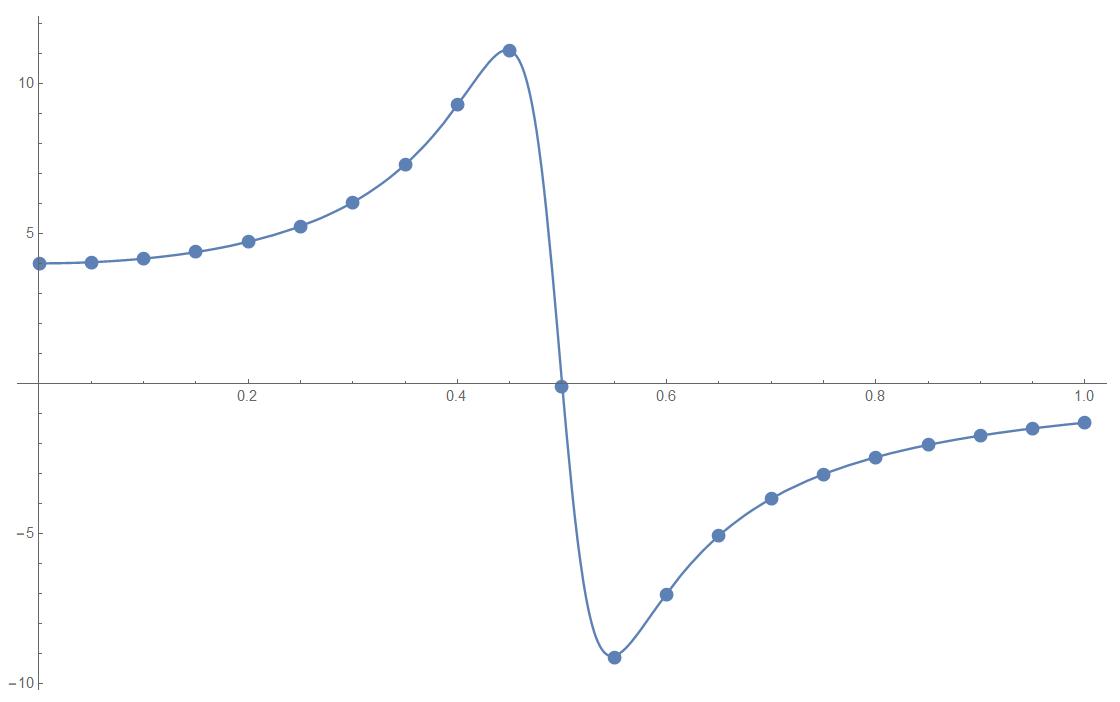
\includegraphics[width=\textwidth]{example-re-epsilon.PNG}
        \subcaption{$\Re \epsilon_\text{r}(\omega)$}
    \end{subfigure}
    \begin{subfigure}{0.45\textwidth}
        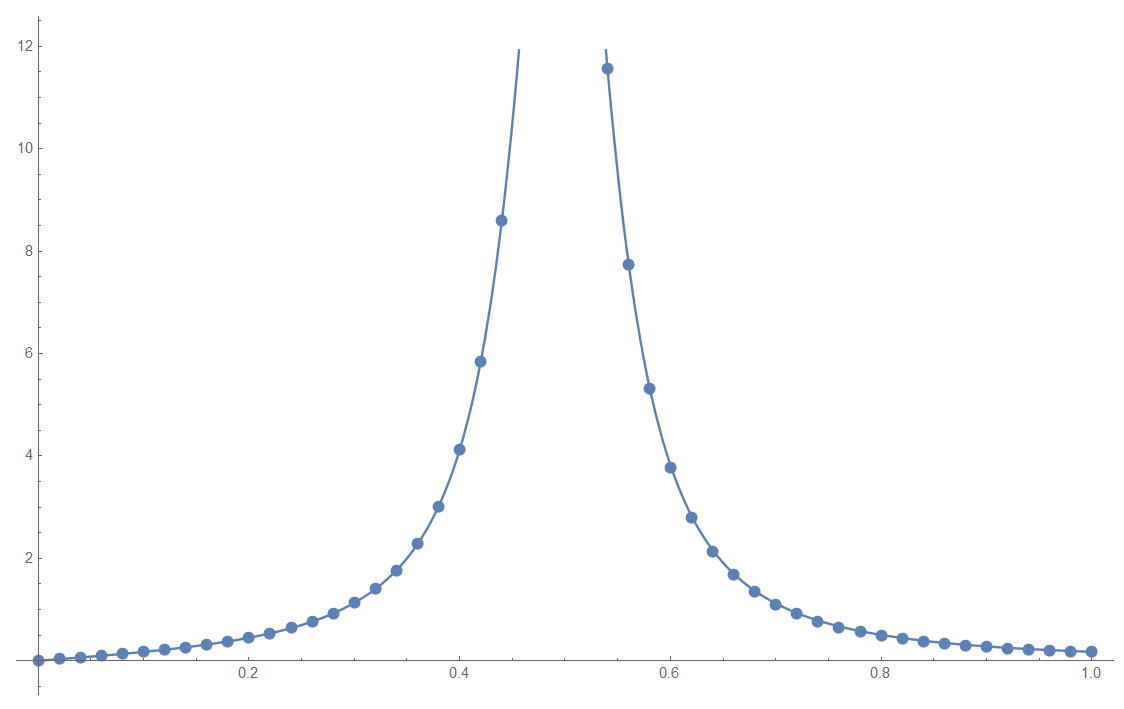
\includegraphics[width=\textwidth]{example-im-epsilon.PNG}
        \subcaption{$\Im \epsilon_\text{r}(\omega)$}
    \end{subfigure}
    \caption{Examples of figures obtained by \href{./homework-2-numerical-a.nb}{\texttt{homework-2-numerical-a.nb}}, where $\omega = 0.5, \gamma = 0.1$, and $L = 50, \epsilon = \num{1e-5}$. The points are obtained by numerically evaluating integrals on RHSs in \eqref{eq:kk-program}, and the curves are obtained by plotting the LHSs in \eqref{eq:kk-program}.}
    \label{fig:demo-curve}
\end{figure}

\begin{figure}
    \centering
    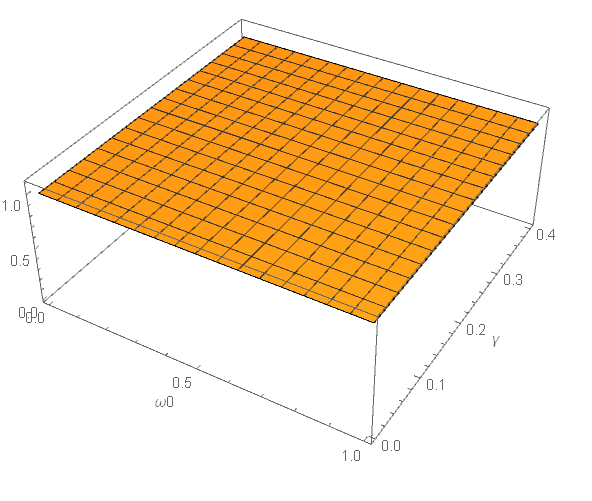
\includegraphics[width=0.6\textwidth]{sum-rule-im-epsilon.PNG}
    \caption{Numerical verification of \eqref{eq:im-epsilon-verify}, where we set $L=60$ and plot the LHS and it is found to always be unity. The code can be found in \href{./homework-2-numerical-c.nb}{\texttt{homework-2-numerical-c.nb}}.}
    \label{fig:im-epsilon-plot}
\end{figure}

\paragraph{}

\paragraph{Ground state with VW term in $G[n]$} 

\end{document}